\documentclass{standalone}
\usepackage{tikz}
\usetikzlibrary{patterns, positioning}

\begin{document}
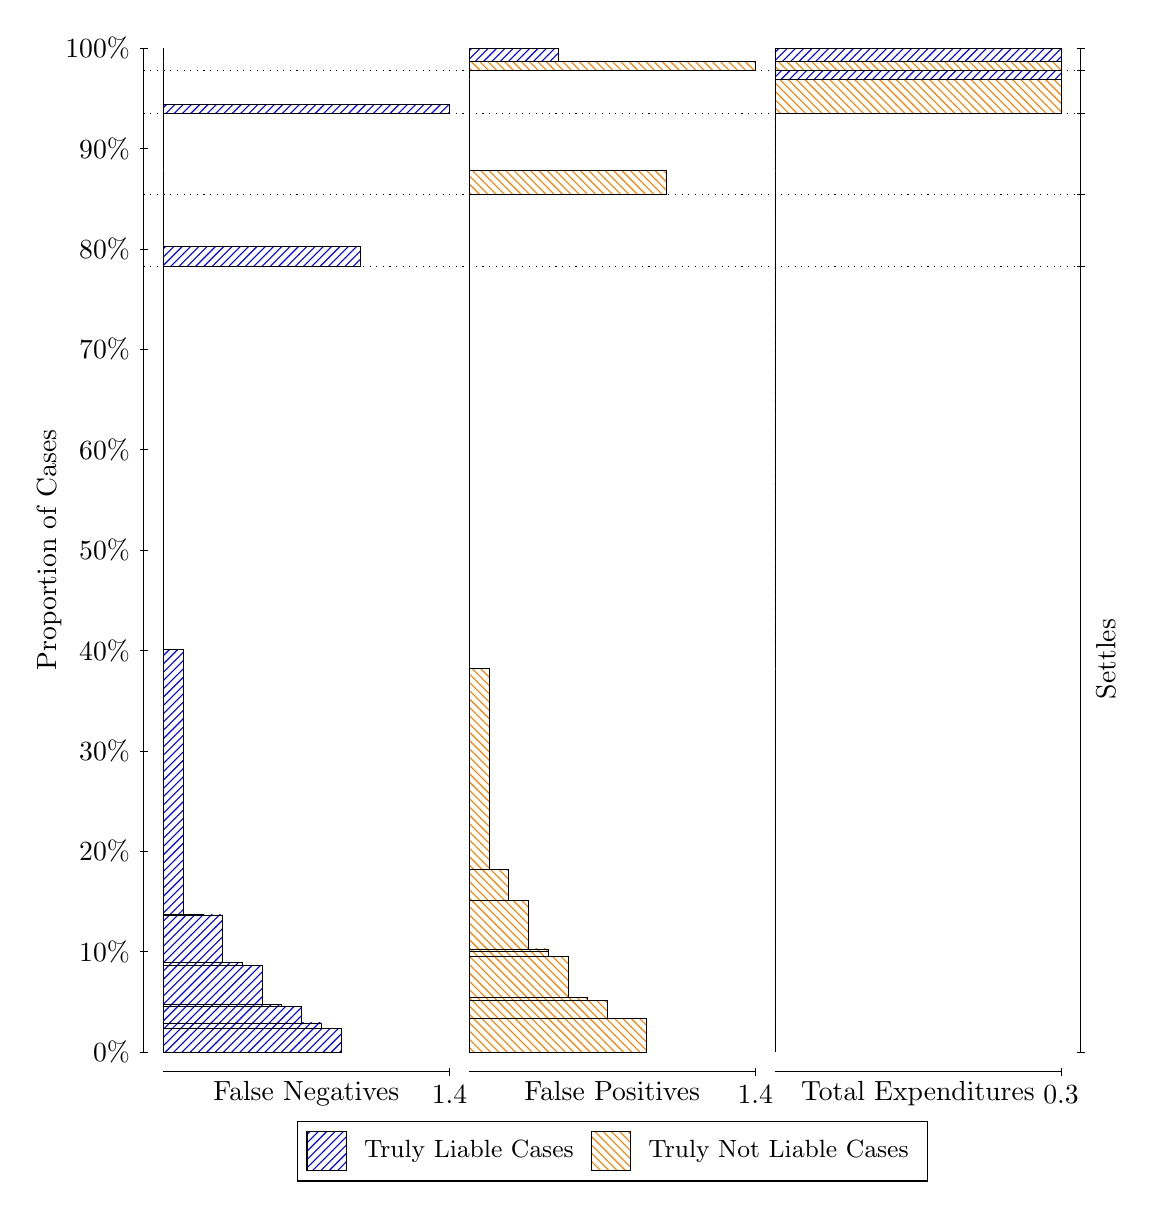
\begin{tikzpicture}
\draw[black, very thin] (1.5,1.75) -- (1.5,14.5);
\node[rotate=90, anchor=center] at (0.3, 8.125) {Proportion of Cases};
\draw[black, very thin] (1.45,1.75) -- (1.55,1.75);
\node[anchor=east] at (1.45, 1.75) {0\%};
\draw[black, very thin] (1.45,3.025) -- (1.55,3.025);
\node[anchor=east] at (1.45, 3.025) {10\%};
\draw[black, very thin] (1.45,4.3) -- (1.55,4.3);
\node[anchor=east] at (1.45, 4.3) {20\%};
\draw[black, very thin] (1.45,5.575) -- (1.55,5.575);
\node[anchor=east] at (1.45, 5.575) {30\%};
\draw[black, very thin] (1.45,6.85) -- (1.55,6.85);
\node[anchor=east] at (1.45, 6.85) {40\%};
\draw[black, very thin] (1.45,8.125) -- (1.55,8.125);
\node[anchor=east] at (1.45, 8.125) {50\%};
\draw[black, very thin] (1.45,9.4) -- (1.55,9.4);
\node[anchor=east] at (1.45, 9.4) {60\%};
\draw[black, very thin] (1.45,10.675) -- (1.55,10.675);
\node[anchor=east] at (1.45, 10.675) {70\%};
\draw[black, very thin] (1.45,11.95) -- (1.55,11.95);
\node[anchor=east] at (1.45, 11.95) {80\%};
\draw[black, very thin] (1.45,13.225) -- (1.55,13.225);
\node[anchor=east] at (1.45, 13.225) {90\%};
\draw[black, very thin] (1.45,14.5) -- (1.55,14.5);
\node[anchor=east] at (1.45, 14.5) {100\%};

\draw[black, very thin] (13.4,1.75) -- (13.4,14.5);
\draw[black, very thin] (13.35,1.75) -- (13.45,1.75);
\node[anchor=west] at (13.35, 1.75) {};
\draw[black, very thin] (13.35,11.729) -- (13.45,11.729);
\node[anchor=west] at (13.35, 11.729) {};
\draw[black, very thin] (13.35,12.642) -- (13.45,12.642);
\node[anchor=west] at (13.35, 12.642) {};
\draw[black, very thin] (13.35,13.67) -- (13.45,13.67);
\node[anchor=west] at (13.35, 13.67) {};
\draw[black, very thin] (13.35,14.214) -- (13.45,14.214);
\node[anchor=west] at (13.35, 14.214) {};
\draw[black, very thin] (13.35,14.5) -- (13.45,14.5);
\node[anchor=west] at (13.35, 14.5) {};

\draw[black, very thin, pattern color=blue, pattern=north east lines] (1.75,1.75) rectangle (4.0052,2.0538);
\draw[black, very thin, pattern color=blue, pattern=north east lines] (1.75,2.0538) rectangle (3.7546,2.119);
\draw[black, very thin, pattern color=blue, pattern=north east lines] (1.75,2.119) rectangle (3.504,2.3246);
\draw[black, very thin, pattern color=blue, pattern=north east lines] (1.75,2.3246) rectangle (3.2534,2.3309);
\draw[black, very thin, pattern color=blue, pattern=north east lines] (1.75,2.3309) rectangle (3.2534,2.3557);
\draw[black, very thin, pattern color=blue, pattern=north east lines] (1.75,2.3557) rectangle (3.0029,2.8451);
\draw[black, very thin, pattern color=blue, pattern=north east lines] (1.75,2.8451) rectangle (2.7523,2.8839);
\draw[black, very thin, pattern color=blue, pattern=north east lines] (1.75,2.8839) rectangle (2.5017,3.4902);
\draw[black, very thin, pattern color=blue, pattern=north east lines] (1.75,3.4902) rectangle (2.2511,3.4982);
\draw[black, very thin, pattern color=blue, pattern=north east lines] (1.75,3.4982) rectangle (2.0006,6.8592);
\draw[black, very thin, pattern color=orange, pattern=north west lines] (1.75,6.8592) rectangle (1.75,11.729);
\draw[black, very thin, pattern color=blue, pattern=north east lines] (1.75,11.729) rectangle (4.2557,11.981);
\draw[black, very thin, pattern color=orange, pattern=north west lines] (1.75,11.981) rectangle (1.75,12.642);
\draw[black, very thin, pattern color=orange, pattern=north west lines] (1.75,12.642) rectangle (1.75,12.943);
\draw[black, very thin, pattern color=blue, pattern=north east lines] (1.75,12.943) rectangle (1.75,13.67);
\draw[black, very thin, pattern color=blue, pattern=north east lines] (1.75,13.67) rectangle (5.3833,13.783);
\draw[black, very thin, pattern color=orange, pattern=north west lines] (1.75,13.783) rectangle (1.75,14.214);
\draw[black, very thin, pattern color=orange, pattern=north west lines] (1.75,14.214) rectangle (1.75,14.327);
\draw[black, very thin, pattern color=blue, pattern=north east lines] (1.75,14.327) rectangle (1.75,14.5);
\draw[black, very thin, pattern color=orange, pattern=north west lines] (5.6333,1.75) rectangle (7.8885,2.176);
\draw[black, very thin, pattern color=orange, pattern=north west lines] (5.6333,2.176) rectangle (7.6379,2.1789);
\draw[black, very thin, pattern color=orange, pattern=north west lines] (5.6333,2.1789) rectangle (7.3874,2.4012);
\draw[black, very thin, pattern color=orange, pattern=north west lines] (5.6333,2.4012) rectangle (7.1368,2.4418);
\draw[black, very thin, pattern color=orange, pattern=north west lines] (5.6333,2.4418) rectangle (6.8862,2.9606);
\draw[black, very thin, pattern color=orange, pattern=north west lines] (5.6333,2.9606) rectangle (6.6356,3.0266);
\draw[black, very thin, pattern color=orange, pattern=north west lines] (5.6333,3.0266) rectangle (6.6356,3.0584);
\draw[black, very thin, pattern color=orange, pattern=north west lines] (5.6333,3.0584) rectangle (6.3851,3.6713);
\draw[black, very thin, pattern color=orange, pattern=north west lines] (5.6333,3.6713) rectangle (6.1345,4.065);
\draw[black, very thin, pattern color=orange, pattern=north west lines] (5.6333,4.065) rectangle (5.8839,6.6198);
\draw[black, very thin, pattern color=blue, pattern=north east lines] (5.6333,6.6198) rectangle (5.6333,11.729);
\draw[black, very thin, pattern color=orange, pattern=north west lines] (5.6333,11.729) rectangle (5.6333,12.39);
\draw[black, very thin, pattern color=blue, pattern=north east lines] (5.6333,12.39) rectangle (5.6333,12.642);
\draw[black, very thin, pattern color=orange, pattern=north west lines] (5.6333,12.642) rectangle (8.1391,12.943);
\draw[black, very thin, pattern color=blue, pattern=north east lines] (5.6333,12.943) rectangle (5.6333,13.67);
\draw[black, very thin, pattern color=orange, pattern=north west lines] (5.6333,13.67) rectangle (5.6333,14.101);
\draw[black, very thin, pattern color=blue, pattern=north east lines] (5.6333,14.101) rectangle (5.6333,14.214);
\draw[black, very thin, pattern color=orange, pattern=north west lines] (5.6333,14.214) rectangle (9.2667,14.327);
\draw[black, very thin, pattern color=blue, pattern=north east lines] (5.6333,14.327) rectangle (6.7609,14.5);
\draw[black, very thin, pattern color=orange, pattern=north west lines] (9.5167,1.75) rectangle (9.5167,6.6198);
\draw[black, very thin, pattern color=blue, pattern=north east lines] (9.5167,6.6198) rectangle (9.5167,11.729);
\draw[black, very thin, pattern color=orange, pattern=north west lines] (9.5167,11.729) rectangle (9.5167,12.39);
\draw[black, very thin, pattern color=blue, pattern=north east lines] (9.5167,12.39) rectangle (9.5167,12.642);
\draw[black, very thin, pattern color=orange, pattern=north west lines] (9.5167,12.642) rectangle (9.5167,12.943);
\draw[black, very thin, pattern color=blue, pattern=north east lines] (9.5167,12.943) rectangle (9.5167,13.67);
\draw[black, very thin, pattern color=orange, pattern=north west lines] (9.5167,13.67) rectangle (13.15,14.101);
\draw[black, very thin, pattern color=blue, pattern=north east lines] (9.5167,14.101) rectangle (13.15,14.214);
\draw[black, very thin, pattern color=orange, pattern=north west lines] (9.5167,14.214) rectangle (13.15,14.327);
\draw[black, very thin, pattern color=blue, pattern=north east lines] (9.5167,14.327) rectangle (13.15,14.5);
\draw[black, dotted] (1.5,11.729) -- (13.4,11.729);
\draw[black, dotted] (1.5,12.642) -- (13.4,12.642);
\draw[black, dotted] (1.5,13.67) -- (13.4,13.67);
\draw[black, dotted] (1.5,14.214) -- (13.4,14.214);
\draw[black, very thin] (1.75,1.5) -- (5.3833,1.5);
\node[anchor=north] at (3.5667, 1.5) {False Negatives};
\draw[black, very thin] (5.3833,1.45) -- (5.3833,1.55);
\node[anchor=north] at (5.3833, 1.45) {1.4};

\draw[black, very thin] (5.6333,1.5) -- (9.2667,1.5);
\node[anchor=north] at (7.45, 1.5) {False Positives};
\draw[black, very thin] (9.2667,1.45) -- (9.2667,1.55);
\node[anchor=north] at (9.2667, 1.45) {1.4};

\draw[black, very thin] (9.5167,1.5) -- (13.15,1.5);
\node[anchor=north] at (11.333, 1.5) {Total Expenditures};
\draw[black, very thin] (13.15,1.45) -- (13.15,1.55);
\node[anchor=north] at (13.15, 1.45) {0.3};

\node[black, centered, rotate=90] at (13.72, 6.7395) {Settles};





\draw (7.449999999999999,1.5) node[draw=none] (baseCoordinate) {};
\begin{scope}[align=center]
        \matrix[scale=0.5, draw=black, below=0.5cm of baseCoordinate, nodes={draw}, column sep=0.1cm]{
            \node[rectangle, draw, minimum width=0.5cm, minimum height=0.5cm, pattern=north east lines, pattern color=blue] {}; &
            \node[draw=none, font=\small] (B) {Truly Liable Cases}; &
            \node[rectangle, draw, minimum width=0.5cm, minimum height=0.5cm, pattern=north west lines, pattern color=orange] {}; &
            \node[draw=none, font=\small] (B) {Truly Not Liable Cases}; \\
            };
\end{scope}

\end{tikzpicture}
\end{document}